\section{Algorithmen}

\begin{frame}
  \frametitle{Kosten beim Hinzufügen eines Tests}
  \begin{description}
    \item[$0$,] falls $\alpha.\gamma\in\pref(H_s)$ und $\beta.\gamma\in\pref(H_s)$. 
    \item[$1$,] falls $\alpha.\gamma\in\pref(H_s)$ und $\beta.\gamma$ erweitert eine bestehende Sequenz in $H_s$ oder umgekehrt.
    \item[$2$,] falls $\alpha.\gamma\not\in\pref(H_s)$ und $\beta.\gamma\not\in\pref(H_s)$, aber beide erweitern je eine bestehende Sequenz in $H_s$.
    \item[$3$,] falls $\alpha.\gamma\in\pref(H_s)$ und $\beta.\gamma$ ist nicht in $\pref(H_s)$ enthalten und erweitert auch keine bestehende Sequenz aus  $H_s$ oder umgekehrt.
    \item[$4$,] falls $\alpha.\gamma$ eine bestehende Sequenz in $H_s$ erweitert und $\beta.\gamma$ nicht in $\pref(H_s)$ enthalten ist und auch keine bestehende Sequenz aus $H_s$ erweitert, oder umgekehrt.
    \item[$5$,] falls sowohl  $\alpha.\gamma$ als auch $\beta.\gamma$ zu neuen Tests führen.
\end{description}
\end{frame}
    
\begin{frame}
  \frametitle{Algorithmus 1}
  \begin{itemize}
    \item Berechne die Mengen $A,B,C$.
    \item Berechne für jedes Paar von unterscheibaren Zuständen unterscheidenden Sequenzen aus den $P_k$-Tabellen:
    Betrachte die erste $P_k$-Tabelle, in denen sich die beiden Zielzustände in verschiedenen Äquivalenzklassen befinden, und berechne unterscheidende Sequenz 'rückwärts'.
    \item Überspringe Paare aus $B$ und $C$, wenn ihre Zielzustände sicherheitsäquivalent sind.
    \item Wähle ein $\gamma$ aus der vorberechneten Menge, sodass die Kosten beim Hinzufügen von $\alpha.\gamma$ und $\beta.\gamma$ minimal sind.
    \item Füge $\alpha.\gamma$ und $\beta.\gamma$ der Testsuite hinzu.
  \end{itemize}
\end{frame}

\begin{frame}
  \frametitle{Präfixrelationssequenzen}
  \begin{figure}
    \begin{subfigure}[c]{0.4\textwidth}
        \centering
        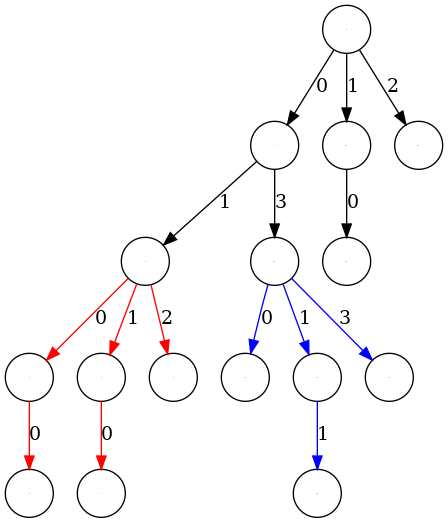
\includegraphics[width=\textwidth,height=5cm,keepaspectratio]{images/PRS_HS}
        \subcaption{Testsuite im Bearbeitungsschritt von $(\alpha,\beta)~=~(0.1,0.3)$.}
    \end{subfigure}
    \begin{subfigure}[c]{0.4\textwidth}
        \centering
        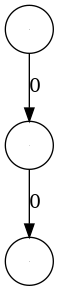
\includegraphics[width=\textwidth,height=5cm,keepaspectratio]{images/PRS_PRS}
        \subcaption{Präfixrelationssequenzen.}
    \end{subfigure}
\end{figure}
\end{frame}

\begin{frame}
  \frametitle{Algorithmus 2}
  \begin{itemize}
    \item Berechne die Mengen $A,B,C$.
    \item Initialisiere Testsuite: $H_s \gets V.\bigcup_{i=1}^{m-n+1}\Sigma_I^i$
    \item Überspringe Paare aus $B$ und $C$, wenn ihre Zielzustände sicherheitsäquivalent sind.
    \item Wähle $\gamma \in PRS(H_s,\alpha,\beta)$.
    \item Falls kein $\gamma$ gefunden werden kann, finde ein Element $x$ aus den PRS, sodass $\alpha.x$ und $\beta.x$ in unterschiedliche Zielzustände führen. Verlängere $x$ zu einer unterscheidenden Sequenz $\gamma$.
    \item Falls kein solches $x$ gefunden werden kann, berechne beliebige unterscheidende Sequenz $\gamma$.
    \item Füge $\alpha.\gamma$ und $\beta.\gamma$ der Testsuite hinzu.
  \end{itemize}
\end{frame}

\begin{frame}
  \frametitle{Algorithmus 3}
  Betrachte Präfixdurchschnittssequenzen
  \begin{itemize}
    \item Durchschnitt zweier Subbäume mit Präfix $\alpha$ bzw. $\beta$ kann immer hinzugefügt werden, ist aber nicht in den PRS enthalten.
    \item Dadurch werden günstige unterscheidende Sequenzen vernachlässigt
    $$PDS = PRS \cup \big( \pref(\successor(\alpha)_{H_s}) \cap \pref(\successor(\beta)_{H_s}) \big) $$
    \item Erhöhter Aufwand
    \item Einziger Unterschied zu Algorithmus 2: Wähle $\gamma \in PDS(H_s,\alpha,\beta)$.
  \end{itemize}
\end{frame}